% Modified
\documentclass{l3proj}
\usepackage{wrapfig}
\begin{document}
\title{Multi-device Recording System}
\author{Alastair Weir \\
        Gordon Adam \\
        Peter Yordanov \\
        Keir Smith \\
        Georgi Dimitrov}
\date{28 March 2014}
\maketitle
\begin{abstract}

Surrounding us in city life there are unqiue moments that are missed by viewing it through the lense of a a smartphone instead of being \'in the moment\' and realising how great the experience could be. This data captured is then restricted to that specific user, letting them only see it from their perspective. By creating a mobile first approach to capturing locational audio centred around these moments, MDRS can crowdsource new insights and perspectives of events in our cities. This aim was successfully achieved with a functioning web and mobile application to allow users to gather this information while still enjoying the moment. Our testing has shown...

\end{abstract}
\educationalconsent
\tableofcontents
%==============================================================================
\chapter{Introduction}
\label{intro}

%==============================================================================
\chapter{Planning}
\label{Planning}

Plans in here will come in handy

%==============================================================================
\chapter{Research}
\label{Research}

Research in here will come in handy

%==============================================================================
\chapter{Design}
\label{design}

The core of our design sprung from early storyboarding and imagined user
profiles which informed us extensively to what a possible system might look
like. As previously discussed, MDRS was viewed as a tool to democratise access
to information at large scale events and share intimate moments or memories of a
place and time through an interactive storytelling medium.

\begin{figure}[ht!]
  \centering
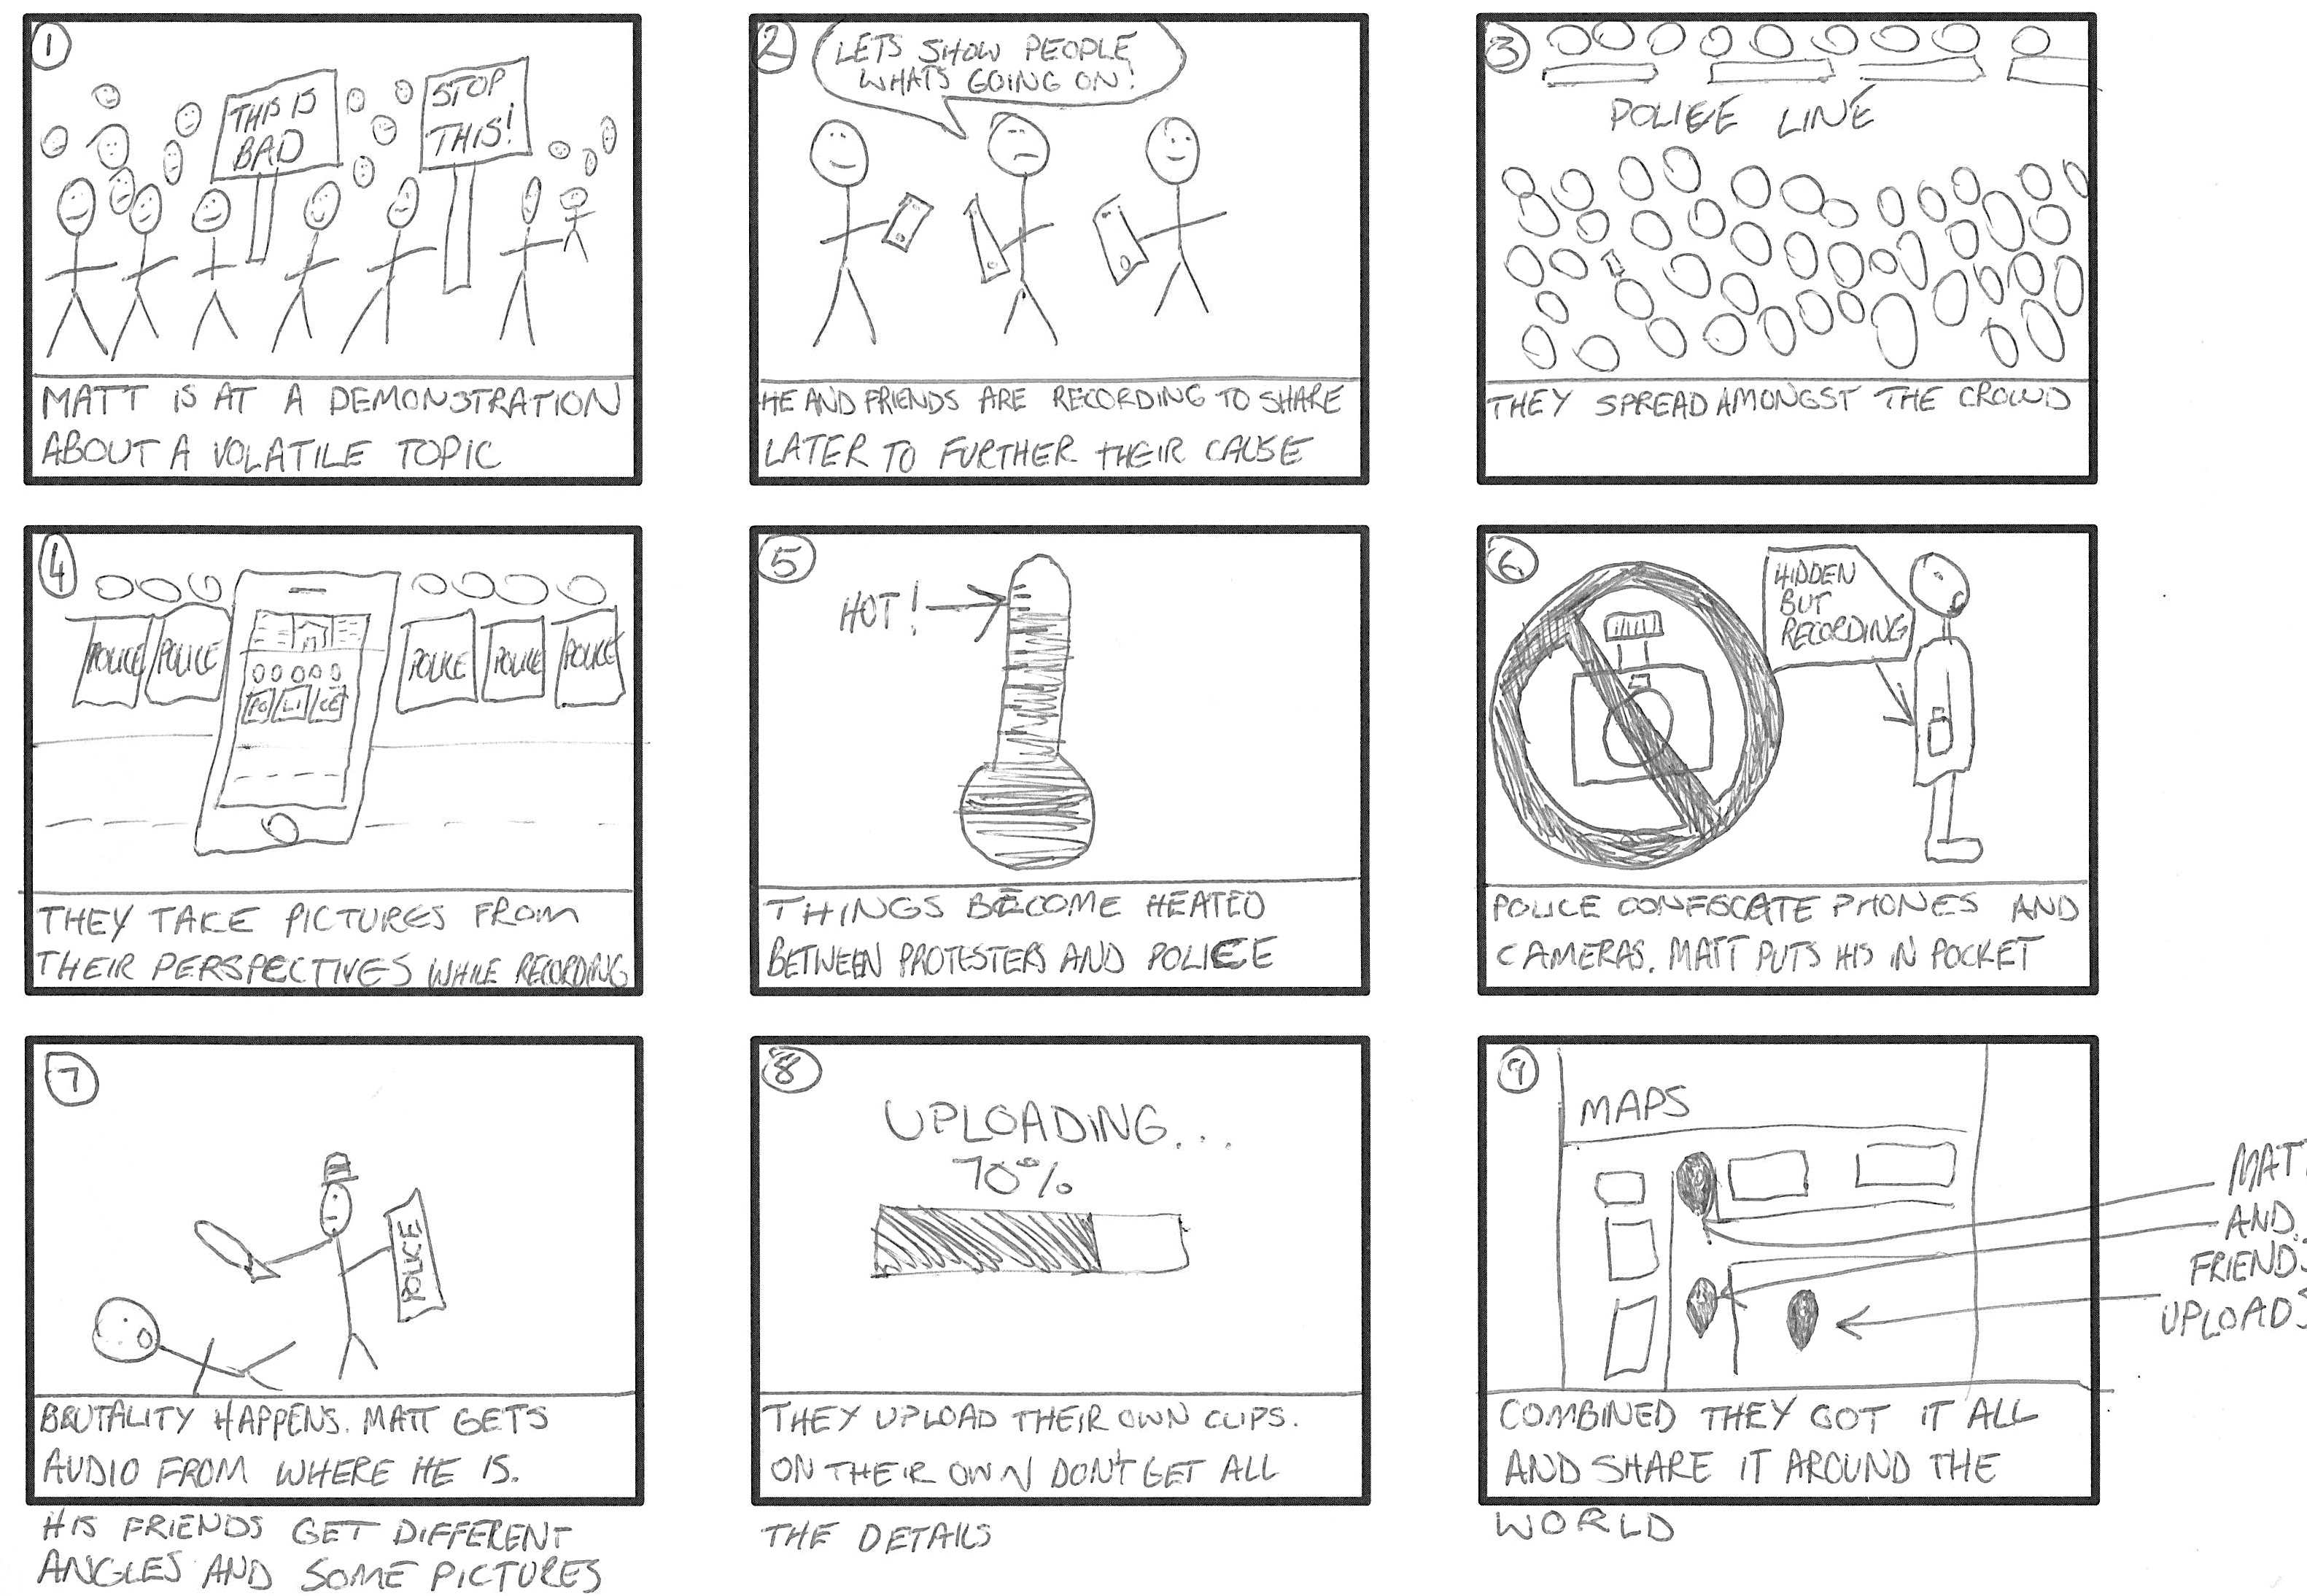
\includegraphics[width=0.75\textwidth]{images/ally-storyboard.jpg}
\caption{Initial storyboard for MDRS.}
\end{figure}
NEED TO ADD MORE IN HERE ABOUT IMAGES ETC {\bf bold}

\section{User Interface}
The realisation that the project would be spread
across both mobile and static devices raised the need for two interaction models
for MDRS was found quickly. For capturing the various forms of data a mobile
implementation was key. Android was quickly chosen as the frontrunner for its
proliferation in the market, an expected ease of development due to its Java
base, which much of the team had experience in, and access to test devices
amongst the team. A web application counterpart was planned for the flexibility
of web technologies which allowed a wide variety of devices and users to access
this facet of the project rather than, for example, a native client for Windows
would.

\subsection{Web Application}   Given the nature of MDRS, the team look to the
Distributed Information Management course taught in second semester as a source
of possible tools. Taught by Leif Azzopardi, the course is structured around the
use of Django, a Python based web framework which would offer us the flexibility
to create a rich, dynamic application easily deployable and widely available to
possible users. Widely used, Django had a wide range of support materials
available including Tango with Django written by Azzopardi and Glasgow
University postgraduate David Maxwell. This resource and knowing we would have
to learn it later through coursework made the framework choice an easy one.

\begin{figure}[ht!]
  \centering
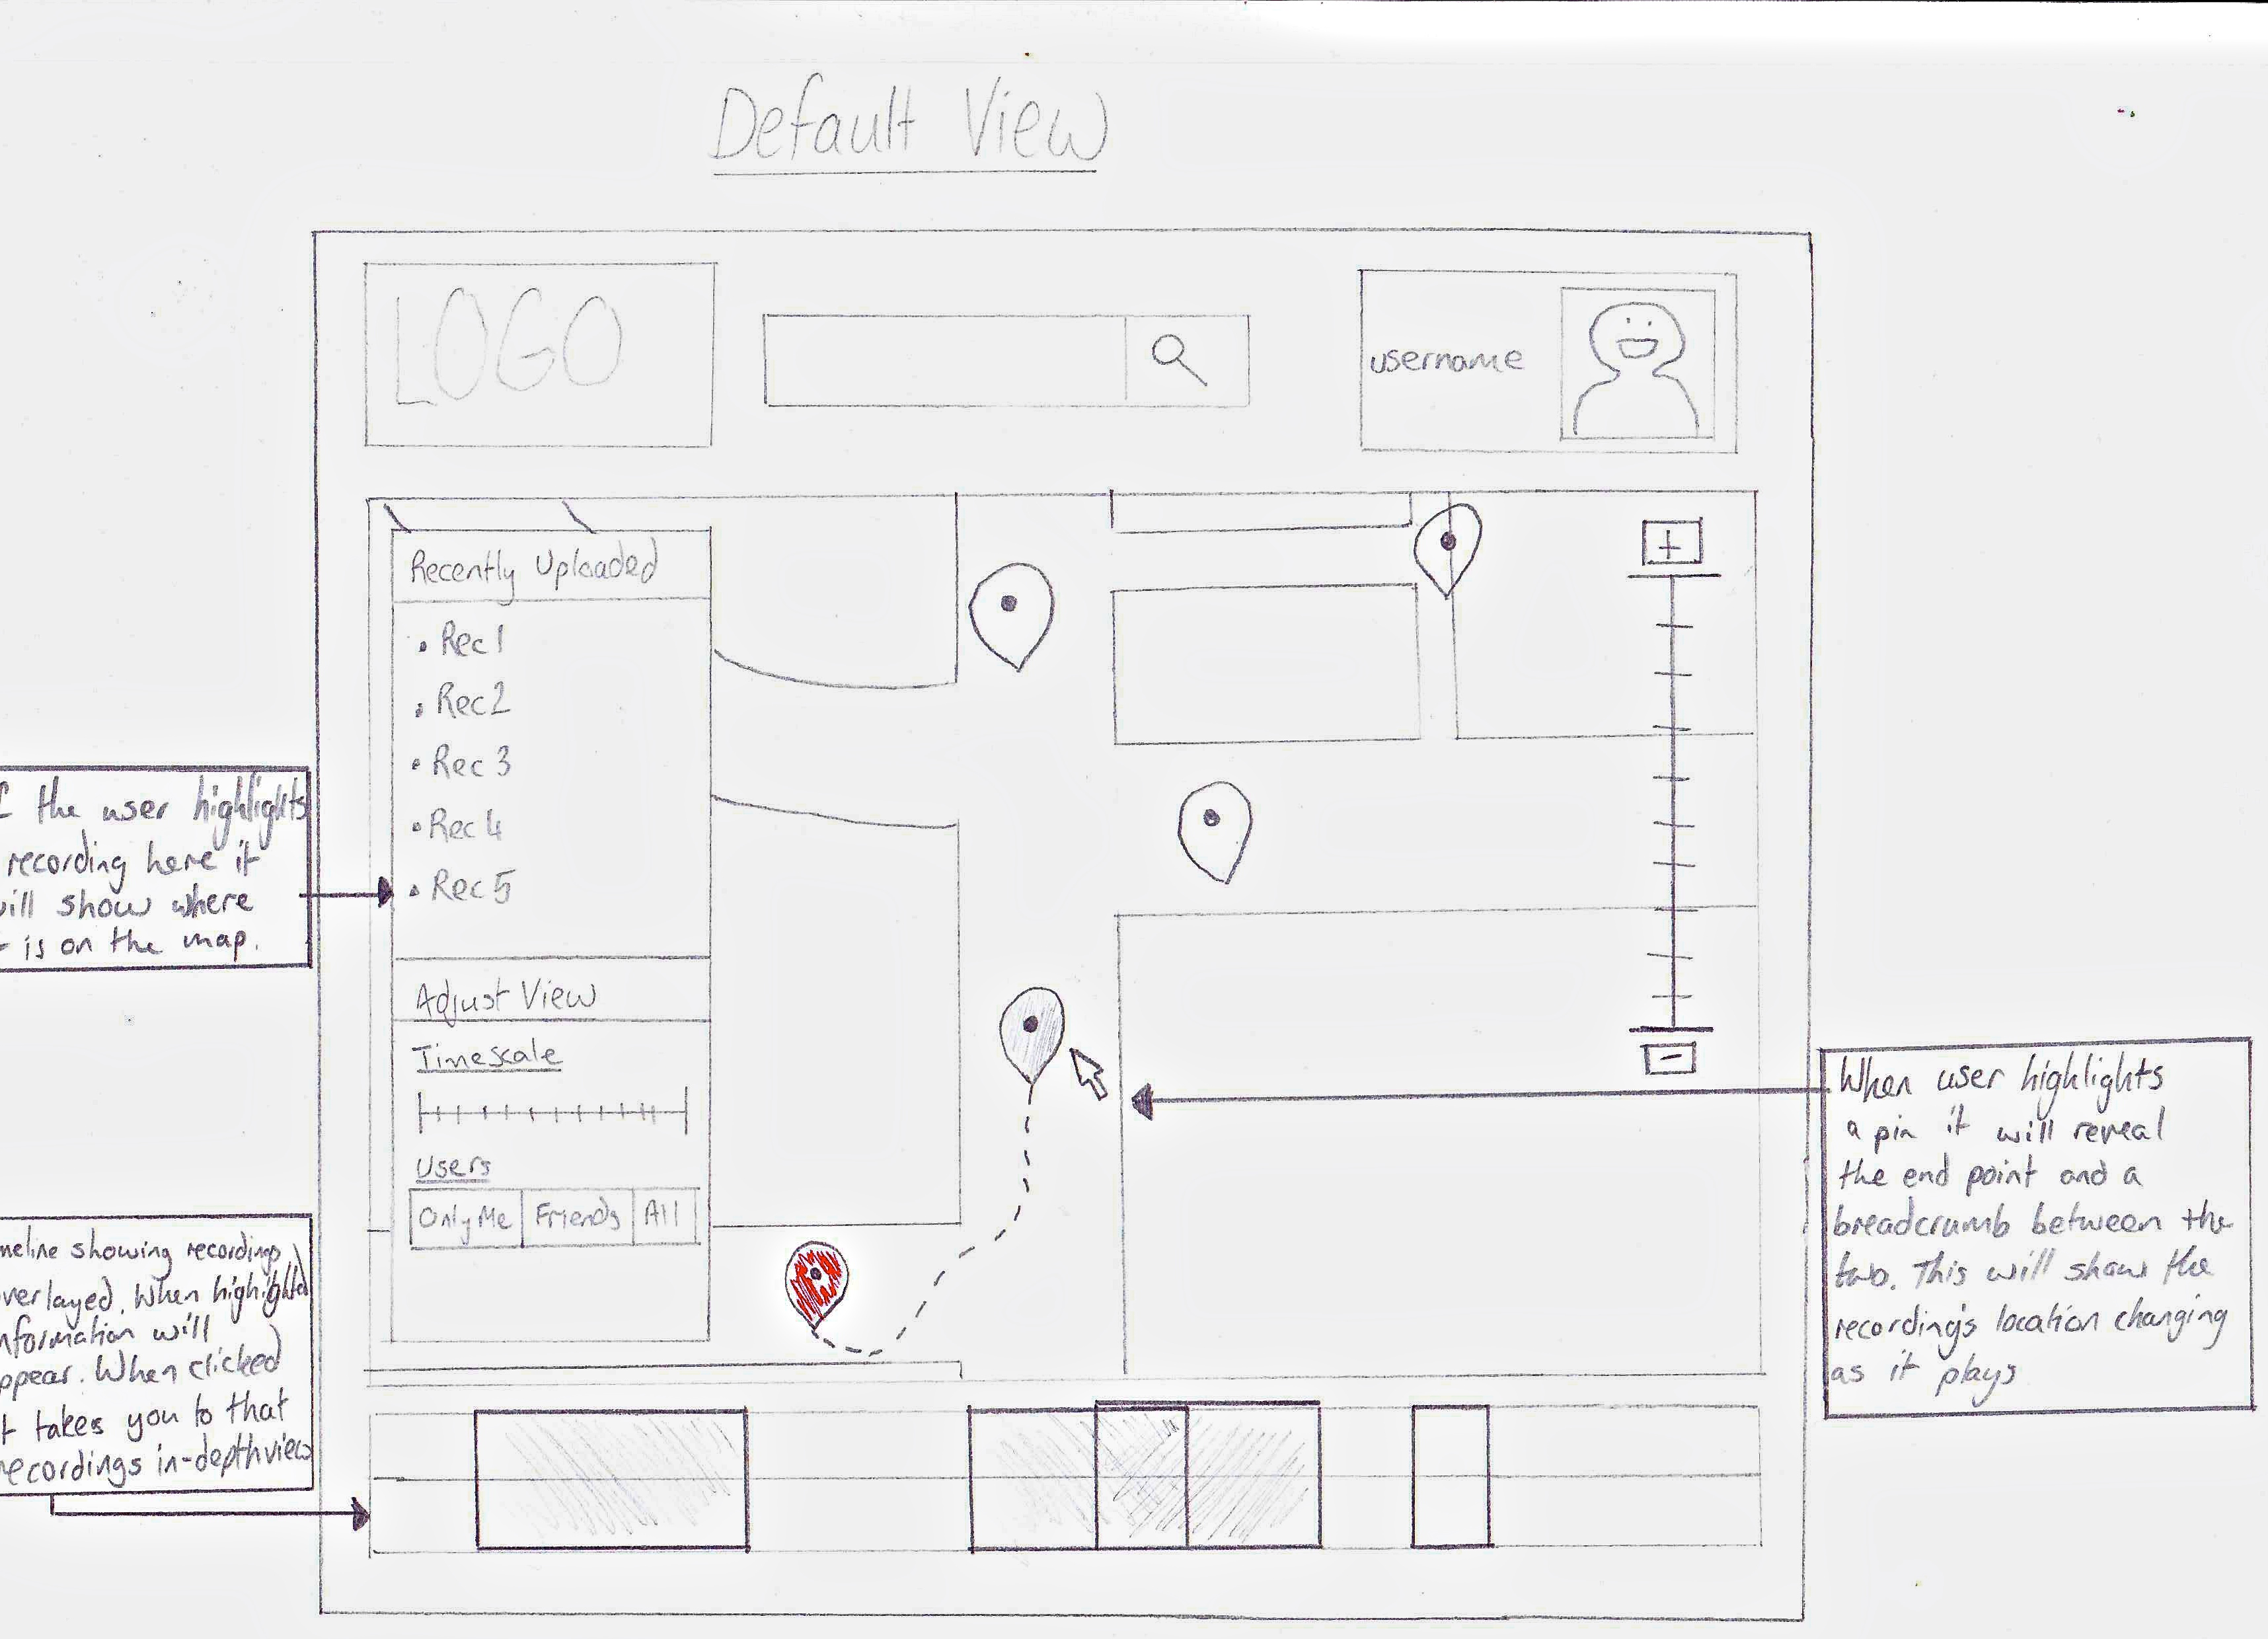
\includegraphics[width=0.75\textwidth]{images/web-map-view.jpg}
\caption{Prototype of map view.}
\end{figure}

The key interaction between the user and MDRS is location therefore it made
sense to make a map the central interface. The user would be able to explore the
map and click on pins representing recordings. This would then project the path
of the recording, indicating where images were captured along the way. Users
could then play it back individually or select multiple recordings for
synchronous playback. With such an important role, the choice of which mapping
API to leverage was extensive in the early stages of the project.

Initially the team were attracted to OpenStreetMap with the very lightweight
Javascript library Leaflet. This would give us unlimited access, as the maps
were open source, but would require us to host the map tiles which amounted to
multiple gigabytes depending on the level of detail chosen. Other disadvantages
were the additional difficulty in initial configuration and setup. Another
option was Microsoft’s Bing maps which didn’t require as much configuration but
were more limited in their free level of access. As an alternative Google Maps
was chosen for its simple API and reasonable access for free users. Ultimately
is offered 100,000 map loads a month for free. We estimated for a typical user
spending 15 minutes on the website that 4 map loads would be needed making this
a workable figure for at least 25,000 user visits a month.

\begin{figure}[ht!]
  \centering
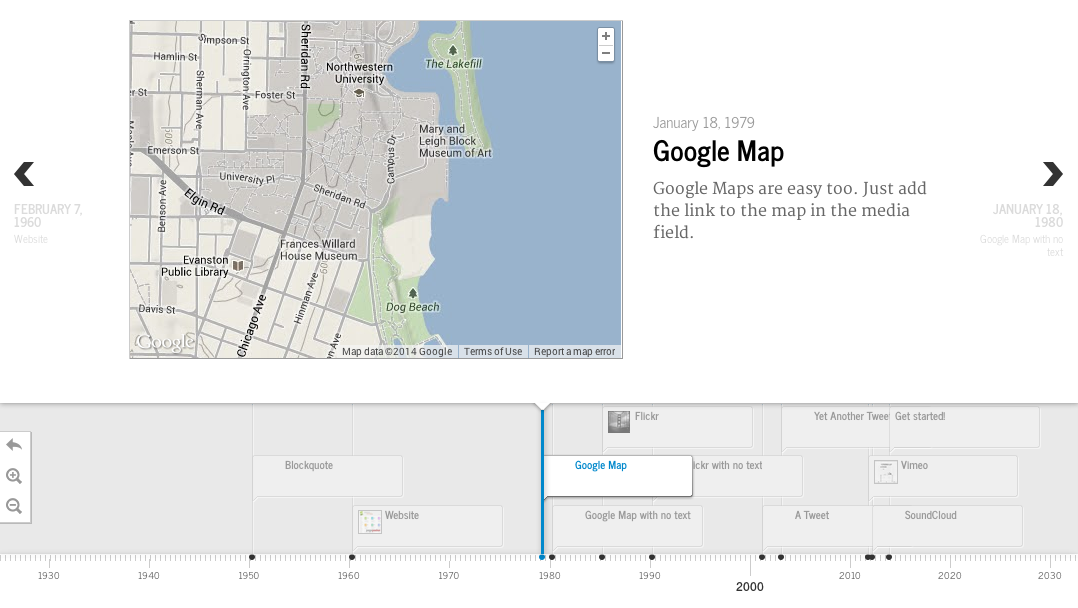
\includegraphics[width=0.5\textwidth]{images/timeline-example.png}
\caption{An example of TimelineJS by KnightLab.}
\end{figure}

A second key component to this interface is the interactive timeline. This was
hoped to show the length of each recording and where they overlapped. Upon
clicking on one a dialog would show its metadata such as name, description, the
user who captured it and accompanying images. Early prototypes also show the
ability to move the current position of playback along the timeline to skip to
different positions. This level of manipulation was simplified upon selection of
TimelineJS which we used to construct it.

Early web interface designs featured a prominent header bar and a floating menu
panel which floated over the map. From early prototypes and wireframes this was
realised to waste a lot of screen real estate, detracting from the reason the
user was on the website. The header bar in particular became wasteful as the
ability to search all recordings was downgraded in importance within the
application. Through discussion in the team it was decided that users would more
likely be interested in audio based on location (the key paradigm of MDRS)
rather than searching through keyword. It gave us a stretch goal to aim for if
development moved along smoothly. Upon research into interface frameworks the
CSS library, PureCSS, was found as a replacement to create an engaging and
simple menu interface. Its simplicity favoured our team’s limited prior
experience with web design and it’s accompanying documentation is excellent.

\begin{figure}[ht!]
  \centering
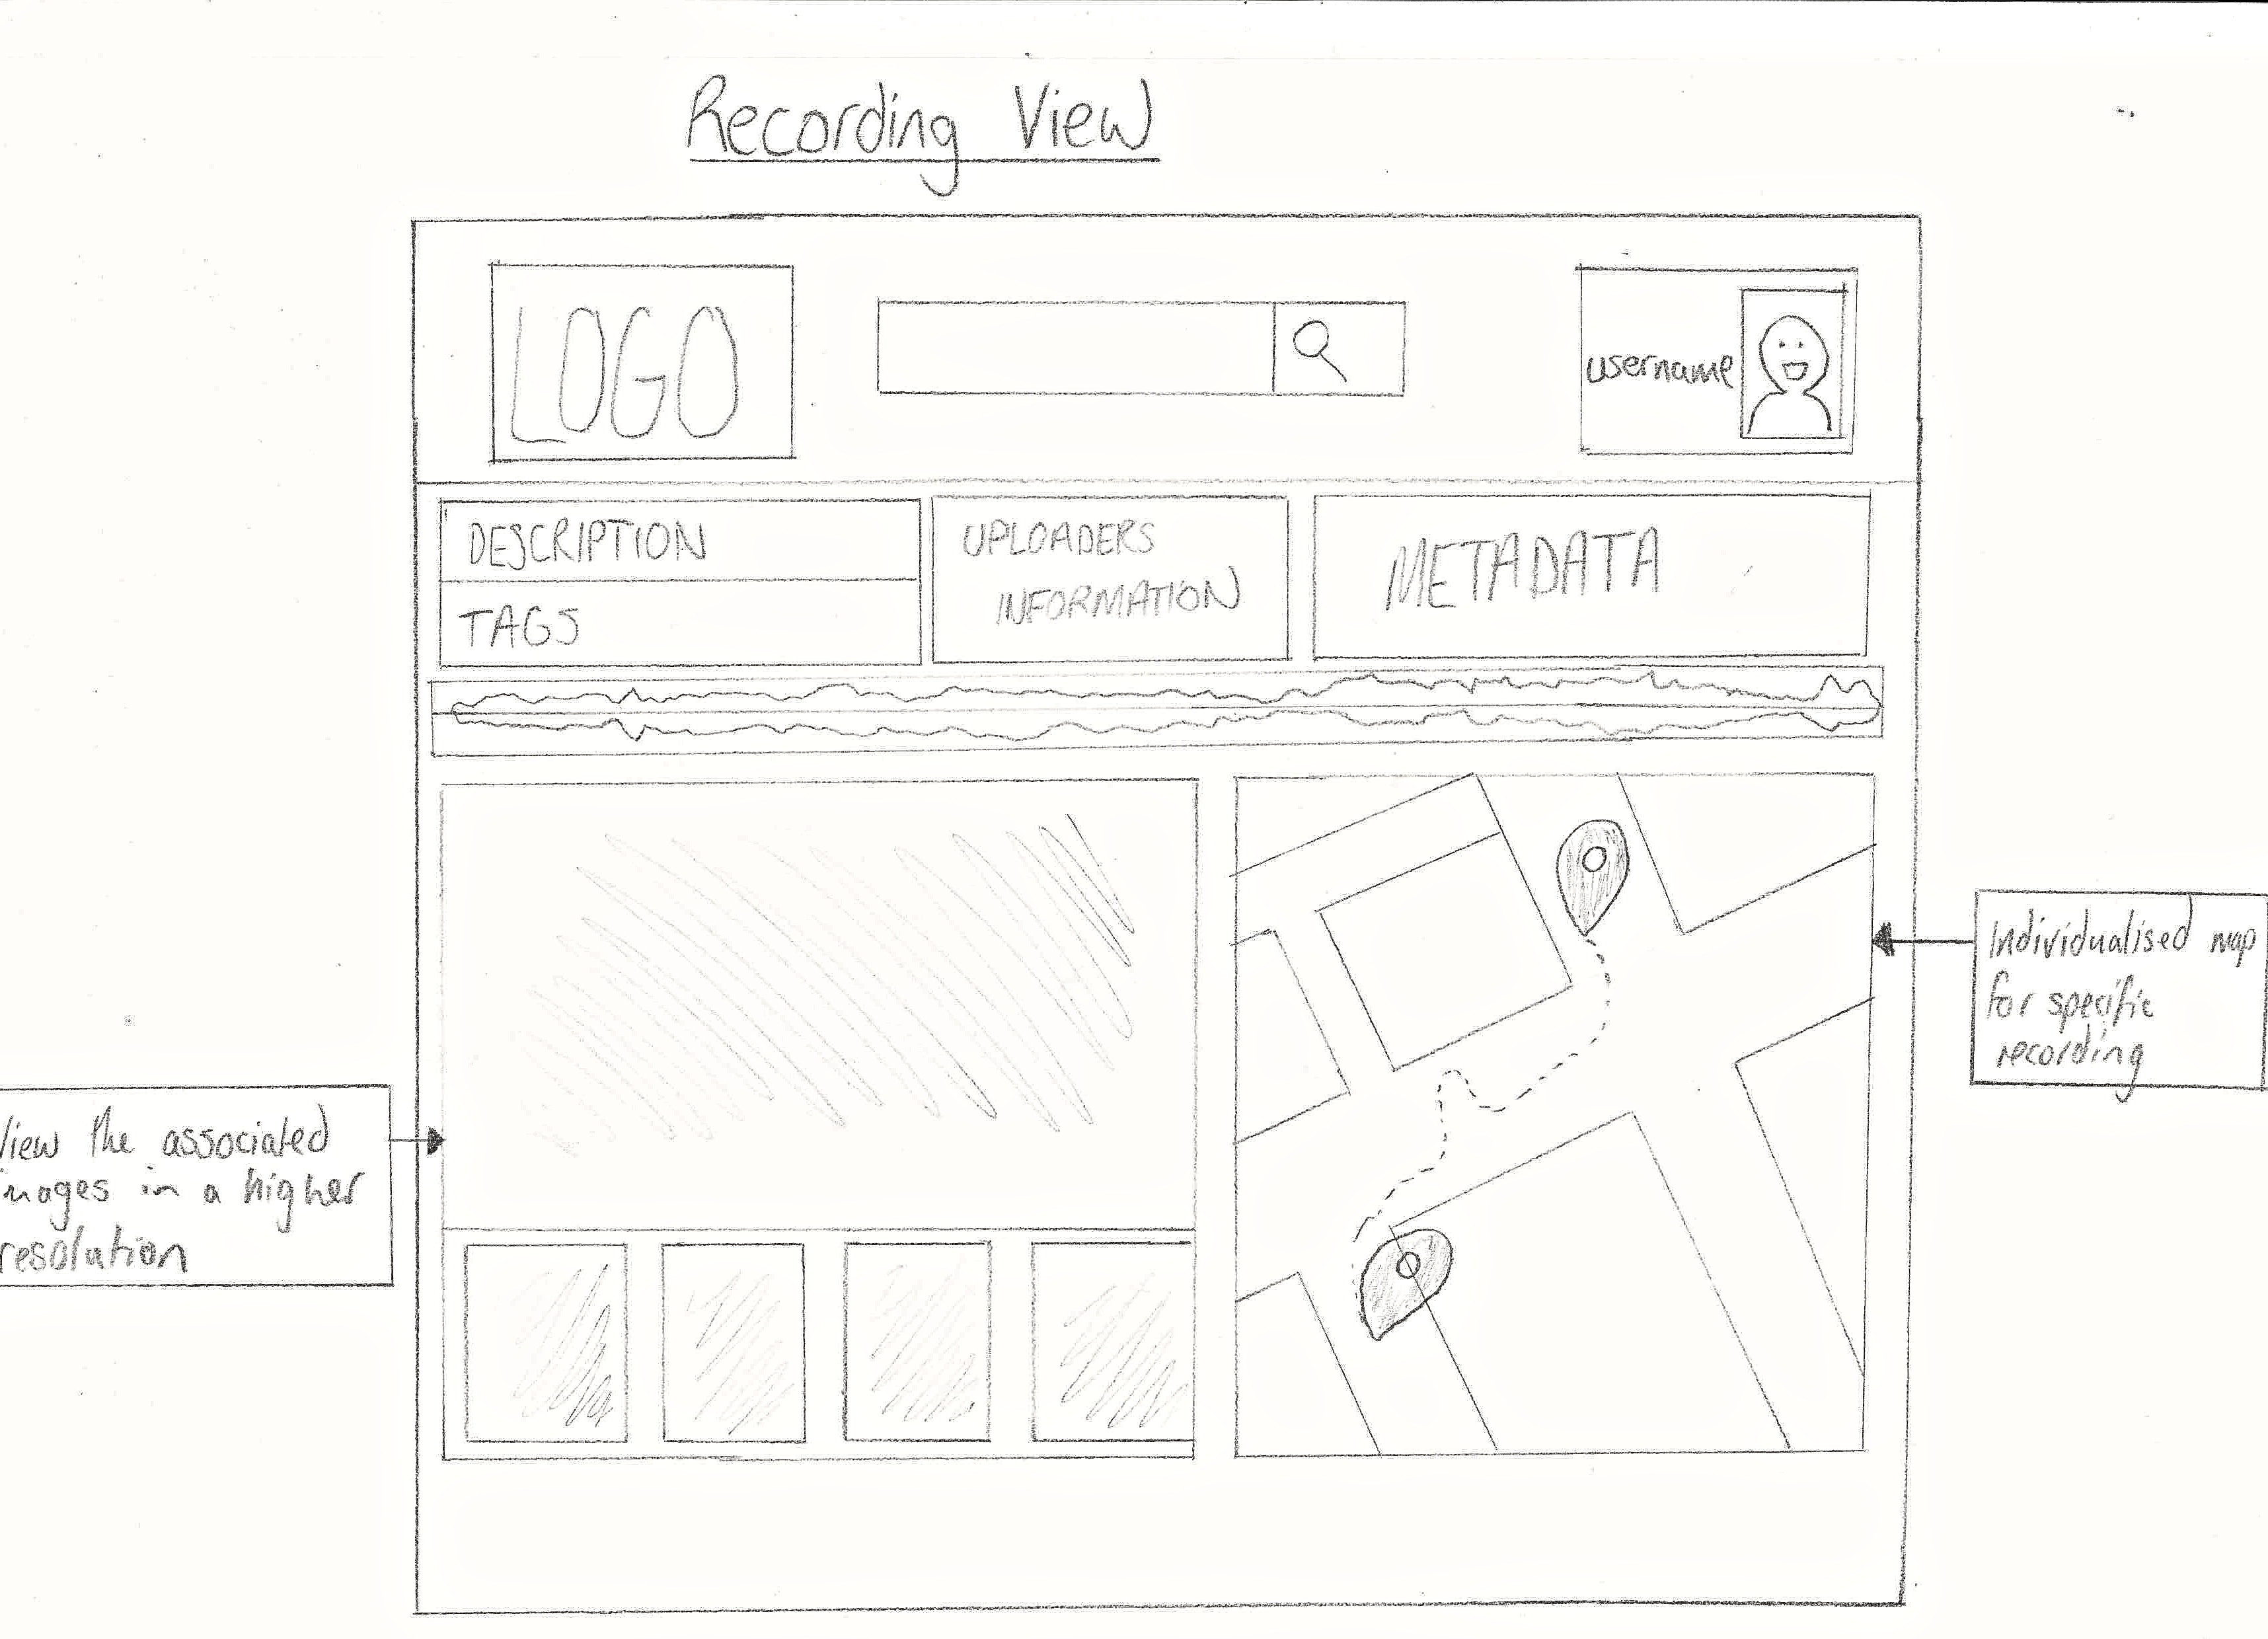
\includegraphics[width=0.5\textwidth]{images/web-recording-view.jpg}
\caption{Recording specific prototype for web application.}
\end{figure}

To accompany this main map view of MDRS was a user page which offered a
personalised insight into a user’s recordings and activity with the application.
It included a personalised timeline and map showing their personal contributions
to the map from which they could play, edit details or delete them from the
service. Along with all the other tools mentioned, the foundations of our
web application’s interface were laid.

\subsection{Android Application} It was decided early on to approach this
element of the project realistically and define a simple set of requirements to
make the application simpler to implement and make the user experience focused
on the core of MDRS, capturing information from the world around us. This meant
it was purely a capture and upload system and it wouldn’t be an alternative to
the desktop viewing interface for interaction with other user’s recordings. Our
focus made the application more achievable while leaving scope for extension in
future development for these playback features.

\begin{wrapfigure}{r}{0.35\textwidth}
  \begin{center}
    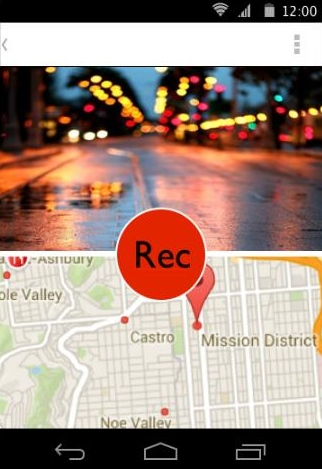
\includegraphics[width=0.34\textwidth]{images/android-digital-prototype-1.jpg}
  \end{center}
  \caption{Initial interface design}
\end{wrapfigure}

In developing an engaging user interface on Android devices, the team looked for
a scalable and intuitive design drawing influence from a wide range of
applications such as Foursquare, Snapchat and Google Play’s suite of
applications while consistently referring to Google’s Android Design Guidelines.
Foursquare was looked to for its integration of a map into a larger whole while
Snapchat’s unconventional, yet intuitive navigation model was seen as a strength
of the application while making an attractive UI. Google’s applications
portrayed the strength and beauty of clear typography and the undeniable rule of
mobile design where less is often more. A utilitarian minimalism through design
was the goal. The core functionality of the application was single use and the
flow through it was clear allowing for a relatively simple approach to be taken,
finding place for flair within the constructs the team placed on themselves.

INSERT INITIAL DESIGN PROTOTYPE HERE

This first UI design offers a split with both a map and view through the camera
lens. The influence for the central record button came from Foursquare’s
prominent placement of their check-in button, placing the key functionality
centrally to draw attention. Downsides to this were its limitations across
smaller screens and a confusing interaction model. Could a user interact and
capture an image before hitting record? This lack of clarity(dw) lead to a
revisionary second prototype.

INSERT SECOND DESIGN PROTOTYPE HERE

This prototype drew more influence from Snapchat’s sliding interface, replacing
its horizontal movement with a vertical one. Again showing the record button on
the divide between a map and camera view, once the record was initiated the map
would slide up bringing up the camera view which would reveal from behind a
frosted glass effect the user’s view into the world they were recording,
prompting them to capture images. This was found very visually appealing and
ended up mostly being used in the final application.


%==============================================================================
\chapter{Implementation}
\label{impl}

In this chapter, we describe how the implemented the system.

%------------------------------------------------------------------------------
\section{Web Application}

Blah blah blah
Blah blah blah
Blah blah blah
Blah blah blah

% - - - - - - - - - - - - - - - - - - - - - - - - - - - - - - - - - - - - - - -
\subsection{Server and Django configuration}

Blah blah blah
Blah blah blah
Blah blah blah
Blah blah blah

%------------------------------------------------------------------------------
\section{Android Application}

\subsection{Early development} With very little experience in developing for
Android, the aim was to take the most key requirements and individually create
demos of each aspect. Then taking all the knowledge gained from this process,
create an application with the must have features, ready to develop it further
if time allowed. d Development Tools) plugin. This reduced the number of new
tools to learn and avoided using unstable software while trying to learn a new
SDK.

Audio recording is key to MDRS' premise so was the first thing to be
implemented. Using Android's MediaRecorder class, a number of demo applications
were prototyped to test audio recording. These repeatedly caused issues and were
by far the longest stage of early development. Consistently the MediaRecorder
would crash the test device (MediaRecorder is not compatible with an emulated
device) with little debug information given by the error logs. Combined with
poor understanding of the Android SDK these tests caused many issues and took up
all Android development time between Mid-November and late December 2013.
Eventually through extensive research surrounding MediaRecorder and learning
more about debugging Android code, the main problem was found to be in
interacting with external storage and the dichotomy between truly external
storage, such as a removeable SD Card, and internal-but-external storage. With
this problem found, the issue was resolved and development could continue.

The next thing to integrate was Google Play Services. This library gives
developers extensive access to many of Google's services such as Maps, In App
Purchases, their Location API, Google+ and Drive. Integrating this library into
the project caused a few issues. While adding a library should be a relatively
simple task, there were wildly varying instructions on how to do this, leading
to a lot of confusion for the team member working on this. Another issue came
down to Eclipse which stores the location of the library's folder on the
computer statically instead of just its path inside the current workspace
directory. This meant when switching between development environments (Windows
and OSX) that it had to be manually updated. Once these kinks were resolved
development could continue to make use of the Maps and Location APIs.

Using Google's excellent documentation for their APIs and the various example
applications on their developer's portal, the initial implementation of the maps
was relatively simple. Making use of the LocationService abstract data type and
using LocationManager allowed the application to gather information from the
device's GPS module or the next most accurate source of positional data. This is
then stored in a LinkedHashMap. Using this data structure allowed the Location
objects collected from LocationService to be stored in a chronological order
with their timestamp acting as each object's key. Parsing this information into
JSON later in the upload process was trivial due to this structured approach at
the data capture stage.

At this stage in development, the basis of what would form the application had
been tested and was found to work roughly as expected. One aspect of development
which had been unplanned was the structure and exact methods required for the
Android application. These first few features were all in one main activity. An
activity in Android is defined as (INSERT A BLOCK QUOTE FROM HERE:
http://developer.android.com/guide/components/activities.html).

REMEMBER TO TALK ABOUT STRUCTURE. HOW I TRIED TO MAKE IT ONE BIG ACTIVITY AND
THEN BROKE IT INTO THREE SUPPORTED BY MULTIPLE CLASSES. IN FUTURE WOULD CHANGE
THIS FURTHER TO BREAK ALL THE ACTIVITIES INTO SUB-ACTIVITIES EFFECTIVELY. BREAK
FUNCTIONALITY OUT INTO THEIR OWN CLASSES.

Google's Android tutorials served as an early touchstone in development,
offering an understanding of an application's structure and layout in
development. An early decision made was to askew the plan to use Google's
Android Studio to use Eclipse with the ADT (Android Development Tools) plugin.

%==============================================================================
\chapter{Evaluation}

We evaluated the project by...

%==============================================================================
\chapter{Challenges}
\label{Challenges}

A number of the challenges we encountered were through a lack of previous
experience and inaccurate expectations held by each member of the team. The
development process offered a lot of flexibility in finding weaknesses in our
ideas and restructuring them forge better working practices and develop new
insights into the workings of a small scale agile team.

\subsection{Technological}

Our main technological issues were over-complication
and over dependence on multiple services for specific channels of communication.
As previously described we embarked on the project with the intention of using a
Redmine instance to keep track of project details, GitHub as our VCS and
Facebook for communication. This convoluted mix made it near impossible to keep
track of discussion about specific issues and problems. While the messaging
component of Facebook was a thoroughly successful choice for social
communication about our Team's work, the group page wasn't as successful. Some
features such as a tracker of who has seen a particular message, it failed due
to posts not being kept in chronological order and no way to easily track
important information.

Through other project work and happenstance, the team discovered GitHub's issue
tracker and wiki features which are individual to each repository. These quickly
became the default means of tracking progress for MDRS, replacing Redmine. The
customisable labels and ability to cross reference issues from commits were
invaluable. GitHub's fast and responsive web interface scaled well across
devices and meant everyone was able to be involved in decisions and contribute
issues to work on. Most of all it succeeded due to the team members being on the
service already whereas Redmine required an intent to go visit it.

Surprisingly email notifications became a great source of information. As
default, GitHub sends out emails for every comment or new issue created. While
filling up inboxes, this device agnostic communication platform made for great
commute reading. While notifications can easily be lost in a endless-scroll, the
emails were small, actionable pieces of key information to keep track of the
project's direction as a whole.

In future, due to the distributed nature of the team and constantly shifting
focus of attention for different deadlines the team would leverage email more.
Weekly status reports would serve as talking points to hopefully make meetings
more productive, giving members time to prepare their thoughts. These would also
serve as evidence of communication and would be easily accessible at a later
date in a chronological order.

Other technological issues revolved around a lack of experience and knowledge at
the beginning of the project. Issues such as handling dependencies from pip with
a requirements.txt poorly made setting up a new virtual environment a challenge.
This was resolved later but mean the team lacked consistency of tools being used
early on.

A major misunderstanding came with the team using VCS. To begin with we did not
understand the workflow of working and testing locally then pushing to the
repository. Initially we were all using SSH to access our server and then
working directly on the server, creating conflicts and locking file issues. This
was quickly resolved when the team researched the issue, quickly changing to the
correct workflow.

\subsection{Organisational}
Our main issue was in poor communication. As
previously discussed we struggled with too many communication channels but this
improved with more face to face interactions in the laboratory and using the
social chat group more for continuous, incremental updates and communication in
the team.

At the beginning of the development cycle, agile roles were assigned for scrum
master, communications with supervisor, librarian and developer. Throughout
development these roles merged and adhered to the agile principles even further.
Due to the ad-hoc nature of the development team and shifting focus amongst
projects, a different team member shifted into the scrum master role who handled
the majority of secretarial jobs, keeping the team on track with tasks assigned
to them to complete. These tasks were assigned taking into consideration each
team member’s strengths and interests. This increased productivity within the
team, pushing our development further and allowing us to expand on the feature
set included in the final project.

%==============================================================================
\chapter{Future Work}
\label{Future Work}

Future work in here will come in handy

%==============================================================================
\chapter{Conclusion}

A great project!

%==============================================================================
\section{Contributions}

Conclusion here

%==============================================================================
\bibliographystyle{plain}
\bibliography{example}
\end{document}
